\chapter{ Realidad aumentada sin marcadores }\label{RASinMarcadores}

\section{Aspectos técnicos}
\subsection{Descripción}
La realidad aumentada es una tecnología que permite mezclar el mundo virtual con el mundo físico, añadiendo la información virtual a la información física ya existente en tiempo real, permitiendo al usuario comprender mejor el entorno que le rodea~\cite{ARCarmigniani}. En la última década, con la aparición de los dispositivos móviles más potentes y las librerías gratuitas de realidad aumentada, el desarrollo de aplicaciones de RA se ha vuelto muy accesible para cualquier desarrollador. Esto implica un aumento drástico en el número de ideas y aplicaciones que surgen día a día.\\

En la actualidad existen tres tipos de seguimiento en la realidad aumentada:
\begin{itemize}
\item \textbf{Realidad aumentada con marcadores (2D y 3D)}: Los marcadores son imágenes impresas, dibujos o objetos previamente escaneados en los que la aplicación reconoce el marcador y activa la experiencia sobre dicho marcador. 

\item \textbf{Realidad aumentada sin marcadores}: Esta es la tecnología más novedosa, ya que combina diferentes tecnologías como SLAM (detallado en el apartado~\ref{SLAMsection}), seguimiento del movimiento, reconocimiento del ambiente o detección de planos para proyectar el objeto y mantenerlo anclado en el mismo punto sin ayuda de ningún marcador.

\item \textbf{Realidad aumentada por geolocalización}: Este tipo de experiencias vinculan a la RA con una ubicación geolocalizada específica. Normalmente se utilizan en exteriores y proporcionan información contextual sobre el ambiente que nos rodea.
\end{itemize}
Las posibilidades de la realidad aumentada sin marcadores están en pleno auge y cada vez aparecen más aplicaciones que mejoran la experiencia de usuario y facilitan el trabajo en algunos sectores como puede ser la industria, la arquitectura, la medicina o la educación.

\newpage
\subsection{Métodos de seguimiento}
El seguimiento (\textit{tracking}) es como conocemos al proceso de localización espacial del usuario en un entorno. Es uno de los aspectos clave en el desarrollo de aplicaciones de realidad aumentada ya que cuanto mejor sea la estimación de la posición y orientación del dispositivo, mejores y más acertados serán los resultados y la inmersión por parte del usuario~\cite{BostanciTrackingMethods}.\\

Los algoritmos de \textit{tracking} se encargan de calcular la posición del dispositivo en relación a los objetos de la escena física. Existen multitud de tecnologías y métodos en los que se apoyan para llevarlos a cabo, siendo los más comunes: sensores mecánicos, magnéticos, sónicos, dinámicos y basados en visión. Hoy en día estos últimos son los más extendidos, ya que la mayoría de los dispositivos desde los que se despliegan las aplicaciones de realidad aumentada, como móviles o tabletas, disponen de una o varias cámaras~\cite{ARToolkit}.\\

El \textit{tracking} basado en cámaras de visión es un subcampo del \textit{tracking} 3D, en el que se utilizan algoritmos de visión por ordenador para obtener de la manera más precisa posible el posicionamiento de seis grados de libertad del dispositivo (tres grados de posición y otros tres de orientación).\\

En este tipo de posicionamiento es necesario disponer de un conjunto de marcadores o referencias tridimensionales para situar la cámara con respecto a ellas. Aunque recientemente se ha tendido a utilizar en menor medida los marcadores físicos para dar una experiencia más rápida y cómoda al usuario, han sido una herramienta imprescindible en los primeros pasos de la realidad aumentada para la obtención de la localización relativa de la cámara.
Según David Marimón~\cite{TrackingThesis}, fundador y director general de Catchoom, se pueden distinguir dos aproximaciones distintas a la hora del tracking: los métodos \textit{Bottom-Up} y los \textit{Top-Down}. 

\subsubsection{\textit{Bottom-Up}}
Las aproximaciones del tipo\textit{ Bottom-Up }pretenden obtener la posición del dispositivo basándose en la información que recibe a través de la cámara.\\

Para este método de \textit{tracking} la posición y orientación se calculan en base a la obtención de características geométricas de objetos y sus relaciones. Dependiendo de los datos procesados, el seguimiento puede ser con marcas o sin ellas.\\

El \textit{tracking} basado en marcas era el método más extendido en los inicios de la realidad aumentada. Hace sus cálculos con la ayuda de marcadores físicos que en su mayoría presentan un gran contraste entre blanco y negro para que los sensores puedan percibirlos con mayor facilidad. Existen también marcadores que usan códigos de colores y diferentes formas geométricas, aunque después de ser sometidos a prueba se comprobó que los más sólidos eran los marcadores cuadrados. Por otra parte, este método es especialmente sensible a la oclusión, ya que cuando se pierde el marcador, es imposible calcular la posición del dispositivo. Por este motivo, se han diseñado algoritmos que pueden hacer frente a este problema mediante estimaciones que completan marcas que no son totalmente visibles.\\

Paralelamente, el \textit{tracking} sin marcas se basa únicamente en las características intrínsecas de la escena, estructuras físicas de fácil percepción como las esquinas de una mesa.\\

Existen técnicas en este campo que utilizan información sobre superficies planas detectadas en el campo de visión, siendo su principal inconveniente su alto coste computacional. De hecho, actualmente este tipo de localización no lo pueden llevar a cabo todos los dispositivos del mercado.\\

Por otra parte, hay técnicas basadas en modelos. No están considerados marcadores porque son parte del medio natural, pero al igual que con éstos los cálculos se basan en el reconocimiento de los objetos que existen y que el programa está preparado para procesar.\\

Finalmente, existen métodos que actúan en escenarios donde no se es capaz de obtener planos o modelos. Sin embargo, estas técnicas no son utilizada habitualmente por sus altos requisitos de cómputo.\\

\subsubsection{\textit{Top-Down}}
Las aproximaciones del tipo \textit{top-down} intentan estimar desde la posición actual del dispositivo si se está percibiendo lo que se esperaba. Es decir, primero se estima la posición y después se confirma esa estimación con los datos del medio.\\

En este caso, se emplean modelos de movimiento para hacer una predicción de la localización del dispositivo. Partiendo de esta estimación, se busca mediante la cámara una serie de referencias parciales que corrijan la predicción y mejoren el posicionamiento del observador. Por ello, todos los modelos \textit{top-down} se ven obligados a trabajar con filtros y modelos de asociación de datos.\\

El uso de estos filtros permite combinar varios métodos de \textit{tracking} y mantener un registro constante de los objetos y la cámara, aunque los marcadores, modelos o planos sean parcialmente visibles por oclusión o se hayan escapado del campo de visión.\\

Además del seguimiento óptico, se han desarrollado numerosas alternativas con las que proporcionar otros métodos de localización (como los \textit{beacons} o la ubicación del GPS) y así complementar y facilitar una localización más precisa y correcta. A las aproximaciones que se valen de varias de estas técnicas se las denomina métodos de fusión.\\

\subsection{Tecnologías implicadas en la RA sin marcadores}\label{tecnologiasImplicadas}
El objetivo de la realidad aumentada es integrar contenido virtual en el mundo real. Idealmente, dicho contenido se tendría que comportar exactamente como uno real, esto requiere una información muy precisa sobre la posición del dispositivo que usa el usuario con respecto al objeto virtual. Para ello, se han desarrollado diferentes tecnologías que junto a los sensores de los teléfonos actuales (giroscopio, acelerómetro, sensor de luz) y a la cámara, permiten disfrutar de una experiencia casi ideal~\cite{ARCarmigniani}. \\

\subsubsection{SLAM (\textit{Simultaneuos localization and mapping})}\label{SLAMsection}
Esta tecnología se basa en una serie de algoritmos complejos que utiliza los datos de los sensores para construir un mapa de un entorno desconocido y a su vez para saber dónde está localizado el dispositivo  \cite{ARCarmigniani}. Esta técnica es usada por robots y por vehículos autónomos. Unos de los ejemplos más presentes en la actualidad son los robots aspiradores, conocidos como \textit{Roomba}.\\

El objetivo principal es saber la localización del usuario en el entorno. En el momento que empiezan los algoritmos, no se tiene ningún tipo de información del entorno. Normalmente, sólo tarda unos pocos segundos en crear un mapa aproximado del entorno con lo que calcula una posición inicial. Más adelante, el mapa creado va creciendo y mejorando en base a la información que obtiene desde el fotograma de la cámara.\\

Aunque este término empezó a aparecer en la década de los 90, las primeras implementaciones carecían de cámaras o sensores que proporcionaban información visual. SLAM estaba pensado para la navegación con robots en entornos desconocidos, hasta que en 2007 Georg Klein y David Murray vieron el potencial de esta tecnología usando sensores visuales en la realidad aumentada~\cite{MaxstMedium}.

\subsubsection{Reconocimiento del ambiente}
Cuanto mejor entienda la aplicación cómo es el entorno que le rodea, mejor será la experiencia del usuario. Por ello, uno de los objetivos principales es el reconocimiento de superficies. El funcionamiento de esta tecnología consiste en procesar cada fotograma obtenido por la cámara y encontrar puntos característicos. Los puntos pueden ser cualquier cosa que ayude a identificar objetos (esquinas, líneas, bordes de objetos, colores, gradientes, etc). En el momento en el que se intenta detectar un plano en una superficie donde el color sea uniforme y carezca de textura o patrones seguramente no funcione con normalidad~\cite{ARCoreConcepts}. Con estos puntos, luego se construye una malla que va a servir como superficie en la escena de nuestra aplicación y con la cual podremos interactuar activándole las físicas y colisión.

\subsubsection{Seguimiento instantáneo}
 El \textit{tracking instantáneo} es una tecnología que no necesita ninguna información previa del entorno para instanciar el objeto, a contrario de la detección de planos. Cuando se empieza el seguimiento, se fija el punto de anclaje y todos los cálculos se realizan con el acelerómetro y el giroscopio, sin procesar apenas la información visual que obtiene de la cámara. Por este motivo, esta tecnología no necesita un alto nivel de luz para funcionar, de hecho EasyAR, una de las librerías que hemos analizado, ni siquiera necesita usar la cámara. La calidad de la experiencia es más pobre frente a la obtenida con reconocimiento de ambiente. 

\subsubsection{Estimación de la luz}
Esta tecnología es muy importante ya que aporta un nivel de detalle excelente, los modelos 3D virtuales se comportan como si fueran reales, se iluminan con la iluminación del mundo físico y emiten sombras en la escena. La estimación de la luz es posible gracias a la combinación de la información del seguimiento del movimiento y usando un algoritmo de análisis de imagen que determina la intensidad de la luz en la imagen del dispositivo. Cuanto más se mueva la cámara y más información recoja sobre el entorno, más precisos serán los datos de dónde viene la mayor fuente de luz, analizando el nivel de brillo de los píxeles de los fotogramas, por lo que se puede estimar la dirección en la que viene. A esta información se puede acceder desde Unity3D o el motor que se use, donde se le aplican los valores obtenidos a una la luz posicional.

\subsubsection{Oclusión}
El término oclusión se refiere a cuando un objeto se deja de ver cuando hay otro objeto o elemento que está en medio de la visión. Para disfrutar de una experiencia de realidad aumentada realista, esta tecnología es esencial, los objetos virtuales tienen que seguir esta regla, porque en el momento en el que cruza una persona delante del objeto, o el usuario pasa la esquina y se sigue viendo el objeto virtual, se arruina la inmersión que podemos llegar a conseguir. Conocer únicamente la posición del usuario respecto al punto de anclaje no es suficiente, es importante saber si existe algún objeto o superficie en medio que nos impide la visión~\cite{articleOclusion}. La implementación de esta tecnología es complicada, por lo que no está presente en muchas librerías.

\subsubsection{Detección de rostros}
Uno de los usos más populares de la realidad aumentada en la actualidad es la detección de caras y su reconocimiento con aplicaciones como Instagram o Snapchat.\\

Cada cara está compuesta por al menos 80 rasgos distinguibles, como la distancia que existe entre los extremos de la mandíbula, la profundidad de las cuencas oculares o la separación que hay entre los agujeros de la nariz~\cite{BBC_FacialRecognition}. Los humanos somos especialmente buenos reconociendo estos rasgos porque tenemos una zona del cerebro dedicada específicamente a interiorizar patrones.\\

Basándose en el funcionamiento del cerebro de una persona se han desarrollado algoritmos que imitan estas asociaciones, dividiendo las caras en un conjunto de puntos de referencia que se llaman \textit{nodal points} y en algunos casos buscando correspondencias con otras fotos tomadas anteriormente. Para tratar de identificar si lo que se  está viendo es una cara se siguen los siguientes pasos: primero se comprueba si existe en la imagen un patrón similar al que formarían los rasgos de una cara, y después se pregunta de quién es esa cara. Sin embargo, no existen dos fotos de una misma persona que sean iguales, de manera que los algoritmos tienen que lidiar con 4 problemas fundamentales a la hora de reconocer la cara de una persona: el envejecimiento, la pose, la iluminación y las emociones.\\

En los últimos años se ha desarrollado un sistema de reconocimiento en 3D llamado \textit{Deepface}, que es capaz de tomar una foto en 2D de un individuo y crear un modelo tridimensional. De esta forma, el sistema tendrá muestras de los rasgos faciales desde todos los ángulos disponibles, solucionando así el problema de la pose.\\

Por otra parte, el problema del envejecimiento también ha sido debidamente prevenido, ya que al crear la estructura 3D de la cara se tienen en cuenta los \textit{nodal points} más importantes y que menos varían con el transcurso de los años, como son las curvas de los ojos, de la nariz o de la barbilla. Pero lo que realmente ha supuesto un avance en este campo es el \textit{deep learning}, un método de \textit{Machine Learning} basado en redes neuronales que guía al programa redirigiéndole si va por mal camino. Cada vez que asocia una cara correcta o incorrectamente, registra el proceso por el que ha pasado para realizar la comprobación y queda guardado en un mapa que va ampliándose sucesivamente con cada acierto o error del sistema. De esta manera, cuantas más conexiones se creen mayor será la fiabilidad a la hora de reconocer una cara.\\

Facebook por ejemplo se vale de este método para el reconocimiento facial y posee una red neuronal de más de 20 millones de nodos, con una fiabilidad del 97.35 \%(datos de 2015)~\cite{Facebook_FacialRecognition} y que aun así es inferior a la capacidad de detección de una persona.\\\

Se espera que con la mejora de la tecnología, el reconocimiento facial sea una forma de identificación tan válida como las huellas dactilares y que puedan identificarse las caras de las personas incluso en grabaciones de seguridad en calidad baja y sin color, así como un método de reconocer el género, edad y otras características del individuo para ofrecerle un servicio o producto más acorde con él en ámbitos como la publicidad.\\

\begin{figure}[H]
     \centering
     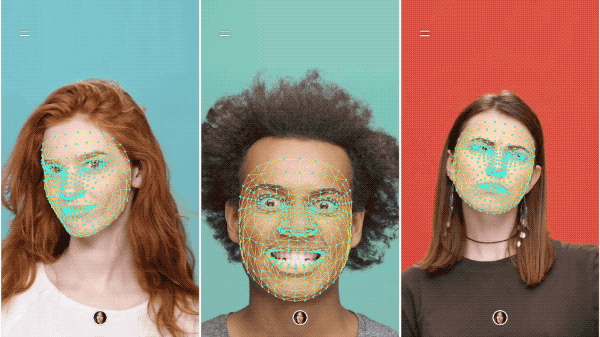
\includegraphics[width=0.7\textwidth]{Images/FaceRecognition.png}
     \caption[Detección de rostros]{Detección de rostros\footnotemark.}
     \label{fig:FaceRecognition}
 \end{figure}
  \footnotetext{Imagen sacada de  \url{https://ai.googleblog.com/2019/03/real-time-ar-self-expression-with.html}}
  
\subsubsection{Puntos de ancla(\textit{Anchor})}
Llamamos punto de anclaje o ancla, a un punto en el mundo real que se usa como referencia en el mundo virtual.\\

En la realidad aumentada tradicional el mecanismo utilizado para situar los objetos virtuales en el espacio real son los marcadores. La cámara identifica el patrón del marcador para  localizar la rotación y posición del objeto en cuestión. Sin embargo, en la realidad aumentada sin marcadores no disponemos de este sistema para guiarnos, de manera que tenemos que buscar otra forma de hacerlo.\\

Una vez localizado el plano o la superficie como explicábamos en secciones anteriores, las librerías de realidad aumentada sin marcadores son capaces de generar un objeto nulo cuya posición servirá como origen de coordenadas. Éste objeto es el llamado punto de ancla o \textit{anchor}, que servirá para colocar objetos virtuales en el mundo físico.\\

Para hacer un buen uso de ellos se debe evitar colocar puntos de anclado en superficies brillantes e intentar que la zona tenga una iluminación buena y consistente.

\subsubsection{Puntos de ancla en la nube (\textit{Cloud Anchor})}\label{cloudAnchorsSection}
El \textit{cloud anchor} es un mecanismo que permite colocar objetos virtuales en una escena de manera que múltiples usuarios puedan interactuar y ver los mismos objetos desde dispositivos distintos. Los objetos colocados pertenecen al mismo lugar físico independientemente del dispositivo que se use para verlo. Su funcionamiento es similar al de los puntos de ancla comunes, que se utilizan para fijar un objeto en una posición, con la diferencia de que los \textit{cloud anchors} se hospedan en los servidores en la nube. De esta manera varios dispositivos pueden consultarlos para situar los objetos en la aplicación.\\

Para ser utilizados, la aplicación en cuestión tiene que tener conexión a internet. Esta tecnología hoy en día sólo está implementada en las librerías ARCore y ARKit. El nombre de \textit{cloud anchors} son actualmente propios del SDK de ARCore, están soportados tanto en Android como en iOS (siempre que el dispositivo lo permita) y funcionan de la siguiente manera: la librería tiene que generar primero un mapa de las proximidades del punto de ancla que será el centro de interés. Para ello, la cámara recopila información y características del entorno cercano desde diferentes ángulos y posiciones durante unos segundos. Cuanto más precisa sea la información recopilada, mejor será la experiencia del usuario. Una vez transcurrido el tiempo, los parámetros del punto se hospedan en la nube y se establece el anchor, devolviendo el servidor un número de identificación único (el \textit{cloud anchor} ID). Cuando otro usuario de la aplicación dirige su cámara hacia el mismo punto de interés, el \textit{cloud anchor} procesa las características visuales del entorno físico desde el nuevo punto de vista. Estas características son comparadas con el mapa 3D que se ha generado anteriormente por el otro dispositivo y se establece la posición y orientación del nuevo usuario con respecto a ello para que pueda ver los objetos virtuales con la mayor precisión posible.\\

Para identificar un punto de ancla en la nube desde otro dispositivo se debe apuntar al lugar en que está situado sin importar la posición del dispositivo, siempre y cuando haya una línea recta entre ambos y no estén separados por una distancia superior a 10 metros.\\

En el caso de ARKit la tecnología para el usuario es igual, pero internamente no funciona de la misma manera. Por temas de privacidad, ARKit no manda los datos a un servidor, si no que utiliza el \textit{framework MultipeerConnectivity} de Apple para mandar la información del mapa (\textit{ARWorldMap}) por una conexión cliente a cliente~\cite{Apple_CloudAnchor}.\\

Cabe mencionar también que los \textit{cloud anchors} tienen una serie de limitaciones en el almacenamiento y el acceso a los datos. En el caso de Google, por ejemplo, sólo se puede acceder a ellos durante las 24 primeras horas después de haber sido colocados y 7 días después cualquier dato en la nube será borrado. El mapa hospedado en la nube no puede ser descargado por ningún usuario y no se puede determinar un lugar geográfico o reconstruir imágenes basándose en el mismo. Además, los datos que envía un dispositivo para que sean comparados con el mapa guardado no se almacenan nunca.\\

\section{Librerías de realidad aumentada sin marcadores}

En este apartado se describirán las principales librerías de realidad aumentada sin marcadores para más tarde estudiar las capacidades y posibilidades particulares de cada una de ellas en el apartado desarrollo.
Por cada librería se recogerán los siguientes datos:
\begin{itemize}
\item Breve descripción
\item Última versión
\item Funciones
\item Plataformas disponibles
\item Tipos de licencia
\end{itemize}
Luego se compararán todas entre sí para resumir las funcionalidades que tienen, las plataformas con las que son compatibles y los lenguajes que soportan.

\subsection{Wikitude}

Desarrollada por Wikitude GmbH, es una de las librerías pioneras en el mundo de la realidad aumentada. Lanzaron su primera aplicación en el 2008, desde entonces, son líderes del mercado. La versión que hemos usado ha sido Wikitude SDK 8.7.0 (2019-08-13)~\cite{Wikitude}.\\

Las principales funcionalidades son:
\begin{itemize}
\item Geo AR (Puntos de anclaje vía GPS)
\item Reconocimiento de imágenes 2D (marcadores) 
\item Reconocimiento de objetos 3D
\end{itemize}

Las plataformas móviles soportadas son:
\begin{itemize}
\item Android
\item iOS
\item Windows
\item Unity
\item Cordova
\item Xamarin
\item Flutter
\item Titanium
\end{itemize}
Soporte para Smart Glasses:
\begin{itemize}
\item Epson Moverio
\item Hololens
\item Vuzix
\end{itemize}
Otras plataformas:
\begin{itemize}
\item React Native
\item Ionic
\item Adobe Air
\item Qt by Felgo
\item LBAR
\end{itemize}
Licencias:
\begin{itemize}
\item SDK Startup. Gratuita para StartUps con menos de dos años de antigüedad y desarrolladores independientes que obtengan menos de 100.000\$ de beneficio en un año.
\item Wikitude Demo. Licencia de 30 días con marca de agua 499€
\item Wikitude SDK PRO (Sólo con marcadores y Geo AR). 1 año de licencia 1990€
\item Wikitude SDK PRO 3D (Paquete completo). 1 año de licencia 2490€
\end{itemize}

\subsection{ARKit}\label{ARKit_Sec}


Esta librería está desarrollada por Apple, fue presentada por primera vez en la Apple Worldwide Developers Conference de 2017.
La versión con la que trabajamos es la ARKit SDK 3.0~\cite{AppleDeve}. A diferencia del resto, para usar esta librería en Unity, no hace falta descargar ningún plugin, viene incluido en el paquete de Unity ARFoundation 2.2.\\

Funcionalidades:
\begin{itemize}
\item Reconocimiento de imágenes 2D (marcadores)
\item Reconocimiento de objetos 3D
\item Reconocimiento de rostro (hasta 3 simultáneamente)
\item Oclusión
\item SLAM
\item Estimación de luces
\item Puntos de anclaje en la nube
\end{itemize}
Las plataformas soportadas son:
\begin{itemize}
\item iOS 
\item Unity (via ARFoundation)
\item Unreal Engine 4~\cite{Unreal}
\end{itemize}
La licencia es gratuita.

\subsection{ARCore}\label{ARCore_Sec}


Esta librería está desarrollada por Google, y fue lanzada en febrero de 2018 como respuesta para competir contra ARKit de iOS. La versión con la que trabajamos es ARCore SDK for Unity v1.11.0 (2019-05-05)~\cite{ARCore}.\\

Funcionalidades:
\begin{itemize}
\item Reconocimiento de imágenes 2D (marcadores)
\item Reconocimiento de objetos 3D
\item Reconocimiento de rostro
\end{itemize}
\begin{itemize}
\item SLAM
\item Mapeado de áreas grandes
\item Estimación de luces
\item Puntos de anclaje en la nube
\end{itemize}
Las plataformas soportadas son:
\begin{itemize}
\item Android (Sólo los dispositivos soportados \cite{ARCoreList})
\item Android NDK
\item Unity (Android, iOS)
\item Unreal Engine 4
\item iOS
\end{itemize}
La licencia para usar ARCore es gratuita.


\subsection{Vuforia}

Esta librería está desarrollada por la empresa PTC. La versión que hemos utilizado ha sido Vuforia SDK Android 8.3.8 (2019-06-13)~\cite{Vuforia}.\\

Funcionalidades:
\begin{itemize}
\item Reconocimiento de imágenes 2D (marcadores)
\item Reconocimiento de objetos 3D
\item Escáner de objetos 3D
\end{itemize}
Plataformas:
\begin{itemize}
\item Android
\item iOS
\item Windows
\item Smart Glasses
\end{itemize}
Licencias:
\begin{itemize}
\item Básica, 42\$ al mes, limita el número de marcadores por licencia a 100.
\item Básica con base de datos en la nube para los marcadores 99\$ al mes.
\item Para la versión pro, la cual incluye marcadores ilimitados, acceso a API avanzada, y soporte en producción. Hay que contactar y hacen presupuesto a medida para la empresa.
\end{itemize}


\subsection{Kudan}


Kudan es una empresa que se dedica al desarrollo de la realidad aumentada, virtual y mixta, además de la conducción autónoma, drones y robots. La versión que hemos utilizado ha sido la Kudan SDK Unity 1.6.0 (2019-07-16)~\cite{Kudan}.\\

Funcionalidades:
\begin{itemize}
\item Reconocimiento de imágenes 2D (marcadores)
\item SLAM
\end{itemize}
Plataformas:
\begin{itemize}
\item Unity (Android, iOS)
\item iOS
\item Android
\end{itemize}
Licencias:
\begin{itemize}
\item AR Indie: Gratis. Pensado para la fase de desarrollo, protegido con marca de agua.
\item AR Business: 1500\$. Para las empresas con menos de un millón de dólares en ingresos.
\item AR Enterprise: Para las empresas con más de un millón de dólares en ingresos, hay que contactar con Kudan y proporcionan un presupuesto personalizado.
\end{itemize}


\subsection{MaxST}



Maxst se fundó en 2010 y se dedica a la investigación y desarrollo de la tecnología de realidad aumentada. Han lanzado Maxst AR SDK, el cual hemos probado en la versión MaxstARSDK\_Unity 4.1.3~\cite{Maxst}.\\

Funcionalidades:
\begin{itemize}
\item Reconocimiento de imágenes 2D (marcadores)
\item Reconocimiento de objetos 3D
\item Reconocimiento de códigos de barras y QR
\end{itemize}
Plataformas:
\begin{itemize}
\item Unity (Android,iOS)
\item Android
\item iOS
\item Windows
\item macOS
\item Epson Moverio BT-300,350 y ODG R-7
\end{itemize}
Licencias:

\begin{itemize}
\item Free. Gratis, para uso no comercial, incluye marca de agua.
\item Pro-one. Para aplicaciones con menos de 100k descargas (no incluye actualizaciones). Pago único de 499\$ 
\item Pro-Subscription. Subscripción anual, incluye actualizaciones 599\$ por año
\item Enterprise. Para aplicaciones con más de 100k de descargas. Hay que contactar con Maxst para recibir un presupuesto.
\end{itemize}


\subsection{8th Wall}


8th Wall desarrolla dos productos diferentes, 8th Wall Web y 8th Wall XR for Unity. El producto que vamos a analizar en el desarrollo es el 8th Wall XR for Unity 11.2.6.519, para que la comparación entre las librerías sea mas precisa, ya que la potencia que tiene en navegador es menor a la que puede llegar a tener una aplicación de Unity~\cite{8thWall}.\\

Funcionalidades:
\begin{itemize}
\item Reconocimiento de imágenes 2D (marcadores)
\item 6 grados de libertad
\item SLAM
\item Estimación de la luz
\end{itemize}

Plataformas:
\begin{itemize}
\item Unity (Android, iOS)
\item Web (A-Frame, BabylonJS, Sumerian, three.js) soportada en la versión web
\end{itemize}
El uso de 8th Wall XR de Unity es gratuito. En el caso de 8th Wall Web, la licencia se cobra según las visitas en la web. Aparte, se necesita una licencia de desarrollador que cuesta 250\$/mes.\\

\begin{table}[H]
    \centering
    \begin{tabular}{c c c c}
    \toprule
        Pago por visita (PPV)&	Paquete estándar&PPV de alto tráfico&Paquete alto tráfico \\
         \midrule
        1000\$/mes	& 3000\$/mes	& 6000\$/mes &	6000\$/mes \\  
 
        0 visitas incluidas &	500k visitas incluidas&	0 visitas incluidas	&5M visitas incluidas\\
 
        0.01\$/visita&	0.01\$/visita extra&	0.0025\$/visita&	0.0025\$/visita extra\\
      \bottomrule
    \end{tabular}
    \caption{Licencias 8th Wall}
    \label{tab:8thwallLicenses}
\end{table}


\\

\subsection{Easy AR}


EasyAR es una compañía china que lleva en el mercado desde 2016. Hemos probado la versión EasyARSense Unity SDK v3.0.1(2019-07-07)~\cite{EasyAR}.\\

Funcionalidades:
\begin{itemize}
\item Reconocimiento de imágenes 2D (marcadores)
\item Reconocimiento de objetos 3D
\item SLAM
\item Grabación de pantalla
\end{itemize}
Plataformas soportadas:
\begin{itemize}
\item Unity (Android, iOS)
\item Android
\item iOS
\item Windows
\end{itemize}
Licencias:
\begin{itemize}
\item EasyAR SDK Basic. Gratis
\item EasyAR SDK Pro, 499\$ por licencia. Añade el reconocimiento de objetos 3D, la grabación de pantalla y reconocimiento de más de un marcador simultáneo.
\item EasyAR SDK Pro trial. Lo mismo que el Pro, pero limitado a 100 usos por día.
\end{itemize}


\subsection{ARFoundation}


Este último no se trata exactamente de una librería, sino de un paquete de Unity (aún en fase experimental) que integra una API de alto nivel (wrapper) que permite tener el mismo código funcional para ARCore y ARKit, según si se compila el proyecto para Android o para iOS. La versión más reciente es ARFoundation 2.2 (Unity 2019.1), incluye las versiones más recientes de ambas librerías~\cite{ARFoundation}.\\

Soporta las mismas funcionalidades que ARCore y ARKit:
\begin{itemize}
\item Reconocimiento de imágenes 2D (marcadores)
\item Reconocimiento de objetos 3D
\item Reconocimiento de rostro 
\item Oclusión (iOS con ARKit)
\item SLAM
\item Mapeado de áreas grandes (ARCore)
\item Estimación de luces
\item Puntos de anclaje en la nube
\end{itemize}

Plataformas soportadas:
\begin{itemize}
\item Unity (Android, iOS)
\end{itemize}

Su licencia, al igual que ARCore y ARKit, es gratuita.
\section{Resumen de características}
\subsection{Tabla de funcionalidades}
A continuación, en la tabla \ref{tab:funcionalidades} se puede ver un resumen de  las funcionalidades que tiene cada una de las librerías que vamos a analizar. Más adelante, en la parte de comparación y análisis de las librerías, evaluaremos la calidad y eficiencia de estas funcionalidades para cada librería.

\begin{table}[H]
\resizebox{\textwidth}{!} {
    \centering
    \begin{tabular}{m{2cm} c c m{2cm} c c c m{2cm}}
    \toprule
        SDK & Marcadores 2D & Marcadores 3D & Tipo tracking & SLAM & Detección de rostro & Estimación de luces & Otras \\
\midrule
\textbf{Wikitude} & \checkmark & \checkmark & Tracking instantáneo & \checkmark & - & \checkmark & Geo AR \\

\textbf{ARKit} & \checkmark & \checkmark & Detección de planos & \checkmark & \checkmark & \checkmark & Oclusión, Cloud Anchor \\

\textbf{ARCore} & \checkmark & \checkmark & Detección de planos & \checkmark & \checkmark & \checkmark & Cloud Anchor \\

\textbf{Vuforia} & \checkmark & \checkmark & Detección de planos & \checkmark & – & \checkmark &  \\

\textbf{Kudan} & \checkmark & - & Tracking instantáneo & \checkmark & - & \checkmark &  \\

\textbf{MaxST} & \checkmark & \checkmark & Tracking instantáneo & \checkmark & – & \checkmark & \\

\textbf{8th Wall XR} & \checkmark & – & Detección de planos & \checkmark & – & \checkmark &  \\

\textbf{EasyAR} & \checkmark & \checkmark & Tracking instantáneo & \checkmark & – & \checkmark & Grabación de pantalla \\

\textbf{AR Foundation} & \checkmark & \checkmark & Detección de planos & \checkmark & \checkmark & \checkmark & \\
\bottomrule
    \end{tabular}
  }
    \caption{Comparación de funcionalidades}
    \label{tab:funcionalidades}
\end{table}
Como vemos en la tabla~\ref{tab:funcionalidades}, menos en el reconocimiento de rostro, casi todas las librerías tienen las mismas funcionalidades, por lo que a priori nos sirve cualquiera para realizar nuestras pruebas de concepto. Por lo que se probarán todas y se verán cuáles son las que mejor resultado proporcionan.

\subsection{Lenguajes y plataformas soportados}

Podemos ver en la tabla~\ref{tab:plataformas} que prácticamente todas las librerías soportan Android e iOS, con lo que podemos deducir que es donde más se está invirtiendo en el mercado. Quizás las \textit{smartglasses} puedan brindar una experiencia de realidad aumentada más agradable, pero todavía está muy lejos de ser accesible para la mayoría de la población, mientras que un dispositivo móvil es mucho más asequible.

\begin{table}[H]
\resizebox{\textwidth}{!} {
    \centering
    \begin{tabular}{c c c c c c c c}
    \toprule
       SDK &	Unity3D (Android, iOS) &	Unreal Engine 4 &	Java &	Objective-C &	C++ & JavaScript \\
       \midrule
Wikitude & \checkmark & – & \checkmark & \checkmark & – & \checkmark \\

ARKit & \checkmark & \checkmark & – & \checkmark & – & – \\

ARCore & \checkmark & \checkmark & \checkmark & \checkmark & – & – \\

Vuforia & \checkmark & – & \checkmark & \checkmark & \checkmark & – \\

Kudan & \checkmark & – & \checkmark & \checkmark & – & – \\

MaxST & \checkmark & – & \checkmark & – & \checkmark & – \\

8th Wall  & \checkmark & – & – & – & – & \checkmark \\

EasyAR & \checkmark & – & \checkmark & \checkmark & \checkmark & – \\

AR Foundation & \checkmark & – & – & – & – & – \\
\bottomrule
    \end{tabular}
  }
    \caption{Comparación de plataformas y lenguajes soportados}
    \label{tab:plataformas}
\end{table}

En la tabla \ref{tab:plataformas}, es muy fácil observar que Unity3D sale ganador, se puede trabajar con absolutamente todas las librerías, además gracias a su editor y entorno visual, resulta muchísimo más cómodo y ahorra mucho tiempo a la hora de desarrollar una aplicación de realidad aumentada.\\

Después de haber analizado las características de éstas librerías de realidad aumentada, en el siguiente capítulo sometemos a cada librería a una prueba para evaluar su funcionamiento.

\section*{Resumen}
Existen diferentes formas de seguimiento en la realidad aumentada: utilizando marcadores, no utilizándolos y basándose en la geolocalización. Estos tipos de seguimiento pueden funcionar de dos maneras. La forma \textit{Bottom-Up} busca calcular la posición del dispositivo en relación a la información que obtiene de la cámara. Esta información puede venir en forma de marcadores físicos, planos, patrones faciales, etc. Por otro lado, la forma \textit{Top-Down} hace una estimación inicial de la posición de la cámara y después con la información que recibe corrige la aproximación previa.\\

En la realidad aumentada sin marcadores se utilizan una serie de tecnologías para calcular la posición de la cámara y los objetos virtuales en la escena física. Algunos de estos métodos son: SLAM, reconocimiento del ambiente, detección de oclusión, detección de rostros y puntos de anclaje.\\

En este capítulo hemos dado un vistazo rápido a las características principales de las librerías de realidad aumentada sin marcadores. En el siguiente capítulo profundizaremos más en el funcionamiento de cada una y las evaluaremos de acuerdo a las pruebas que hemos realizado.

\noindent